Die Architecture Governance ist dafür verantwortlich sicherzustellen, dass die Enterprise Architecture konsistent in allen Projekten eingehalten wird. Im Bezug auf das Datacenter und die darin laufenden Anwendungen bedeutet das kontinuierlich bestimmte Aspekte zu überwachen.

Entscheidende Aspekte die überwacht werden sollten sind Metriken, wie zB. die Auslastung des Datacenters oder einzelner Komponenten, sowie Anwendungsspezifische Metriken, die sich aus der Natur der Anwendung ergeben. Auch die Compliance der Anwendungen mit den Vorgaben und Richtlinien der Enterprise Architecture, sowie die Einhaltung von definierten Prozessen (zB. Migrierung) sollten kontinuierlich überwacht werden. Bei Veränderungen im Datacenter, beispielsweise durch Skalierung und Erweiterung sollte durch Beobachtung sichergestellt werden, dass diese mit den Businesszielen einhergehen. 

Metriken können sehr hilfreich dabei sein Richtungen für Verbesserungen zu finden. Beispielsweise bei zu niedriger oder zu hoher Auslastung des Datacenters sollte über eine entsprechende Skalierung nachgedacht werden.

\begin{figure}
	\centering
	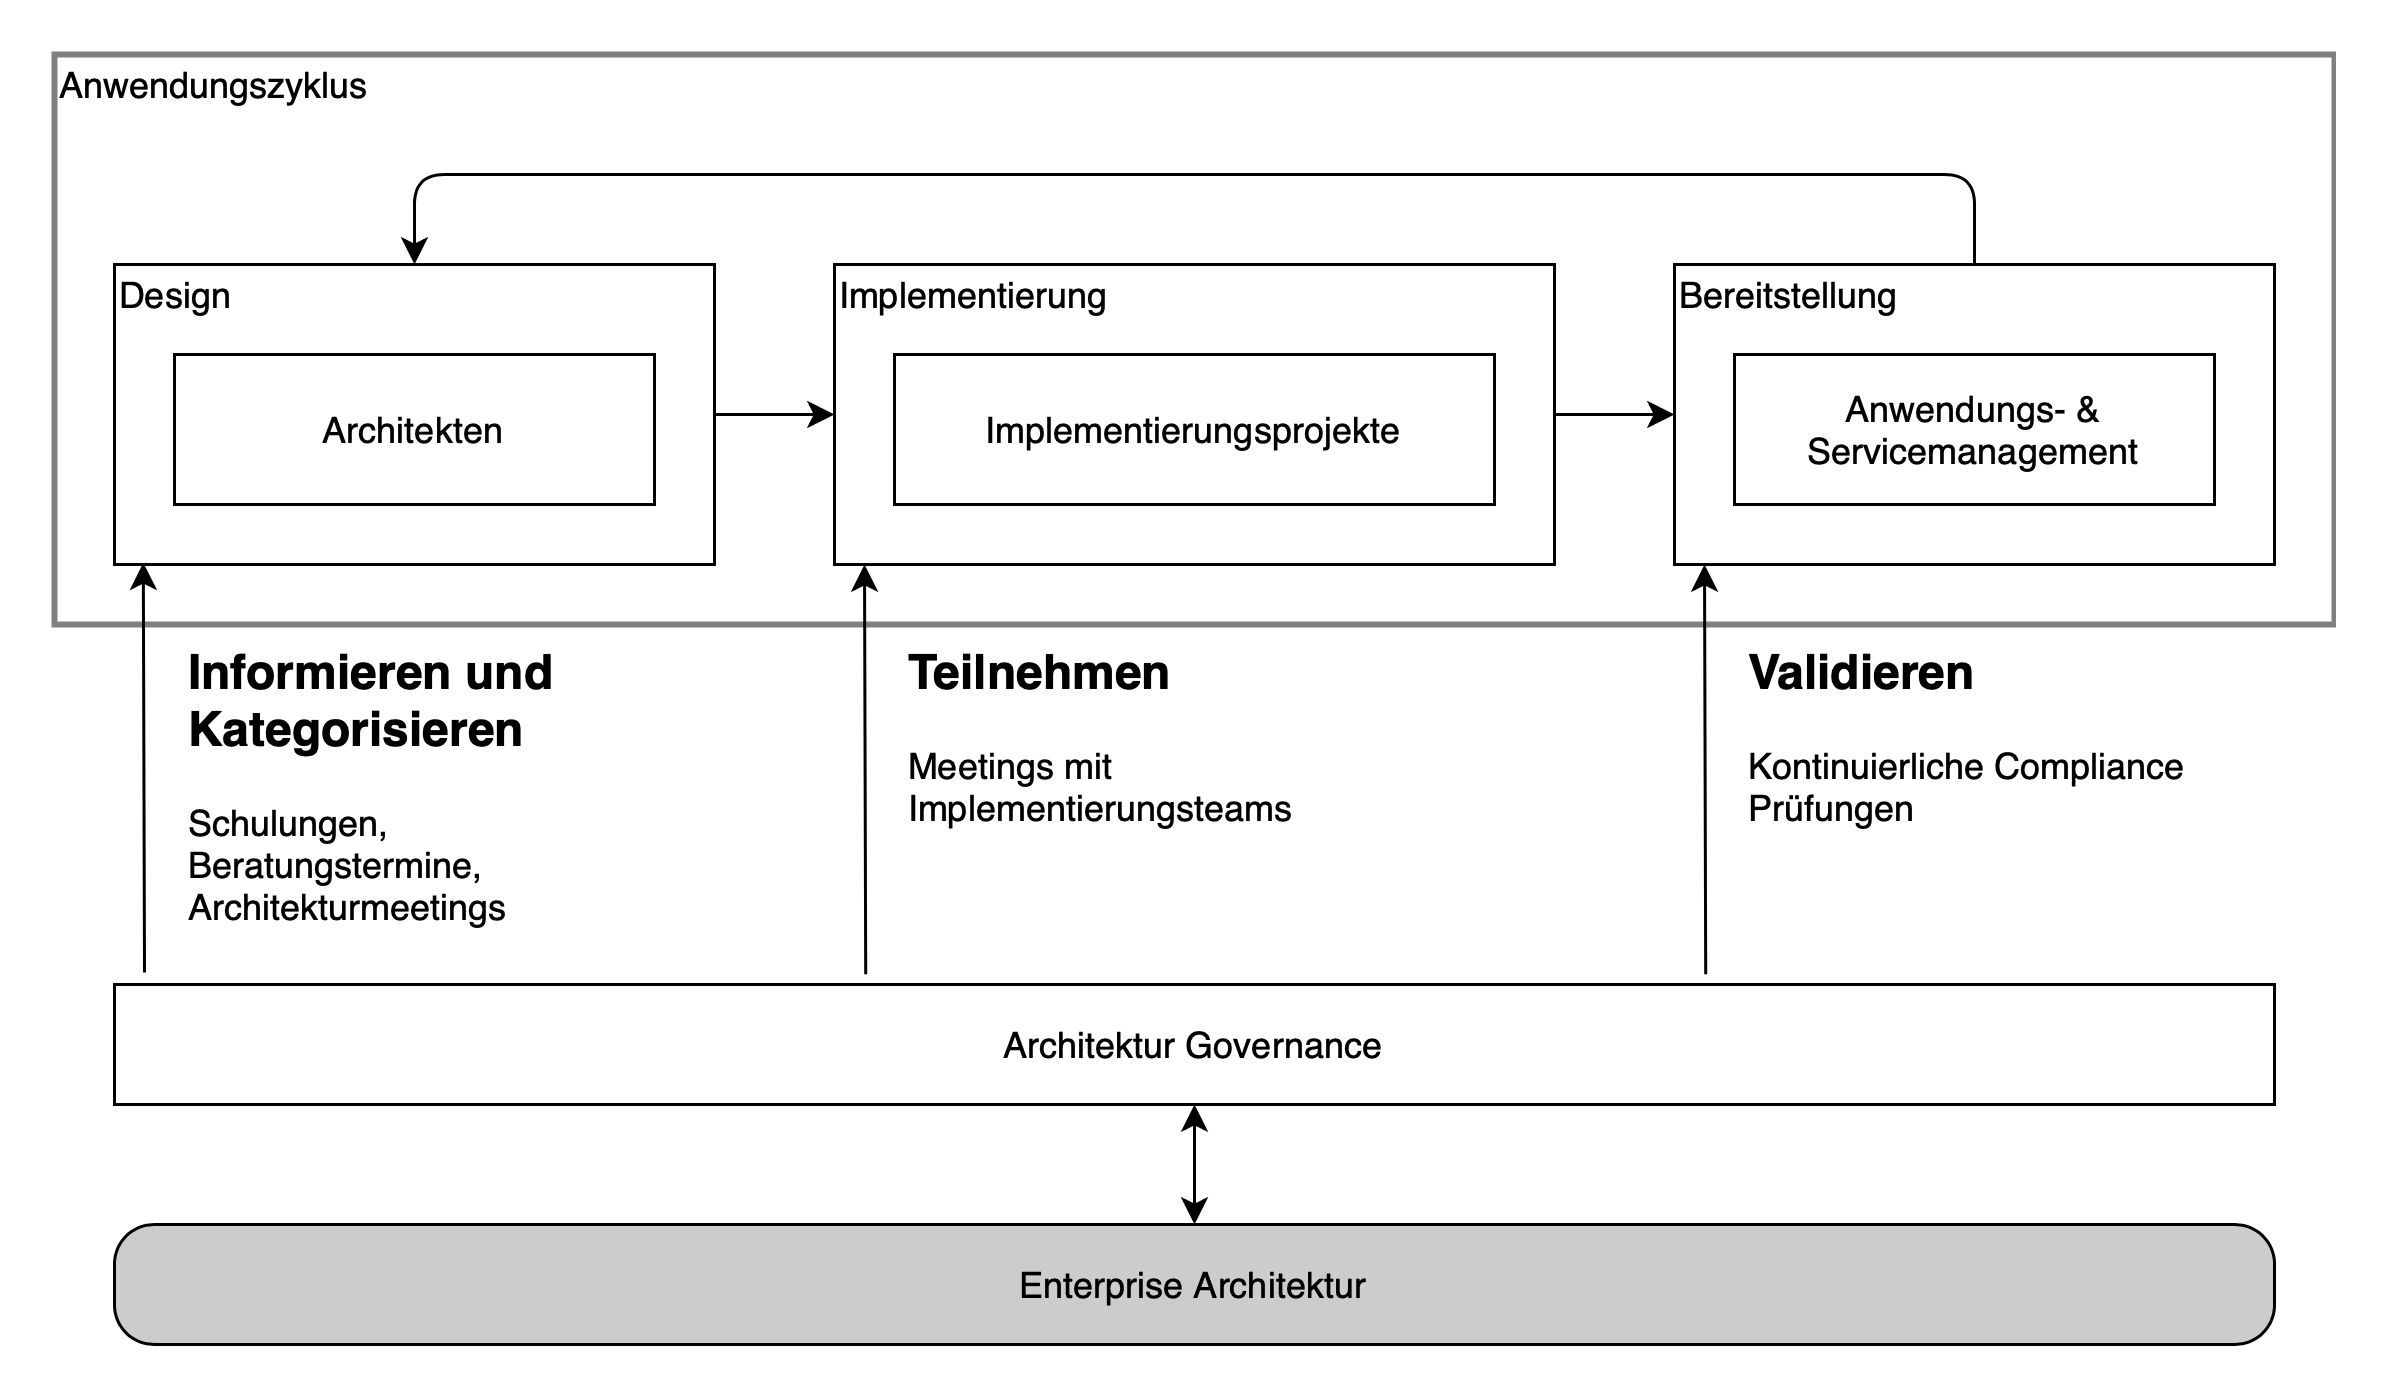
\includegraphics[width=\linewidth]{img/governance}
	\caption{Prozessübersicht der Architecture Governance}
	\label{fig:governance}
\end{figure}

Einer der wichtigsten Aufgaben der Architecture Governance ist es den Anwendungszyklus zu überwachen. Diese Aufgabe lässt sich in vier Teile unterteilen:

\begin{itemize}
	\item Informieren
	\item Projekte Kategorisieren
	\item An Entwicklung teilnehmen
	\item Validieren
\end{itemize}

Über die drei Phasen des Anwendungszyklus (Design, Implementierung, Bereitstellung) hinweg, ist die Architecture Governance konstant beteiligt. In der Designphase sollte es Angebote für Beratungstermine und Schulungen für Architekten geben, um sie mit der Enterprise Architecture vertraut zu machen und sie bei der Gestaltung der Anwendung in Übereinstimmung mit den Vorgaben zu unterstützen. In der Implementierungsphase sollte es fortlaufend Meetings mit den Implementierungsteams geben um sicherzustellen, dass die Anwendung nicht von den Vorgaben abweicht. In der Bereitstellugnsphase müssen bereitgestellte Anwendung kontinuierlich auf Compliance überprüft werden. Da die Bereitstellungsphase direkt zurück zur Designphase führt müssen eventuelle Änderungen der Architektur, die Änderungen an Anwendungen erforderlich machen sowohl hier, als auch in der Designphase kommuniziert werden. Auch müssen in der Bereitstellungsphase die Metriken der Anwendung überwacht werden.